\clearpage
\section*{4. Implementation}
\label{sec:implementation}
\subsection*{4.1 Structural design and responsibilities}

\begin{center}
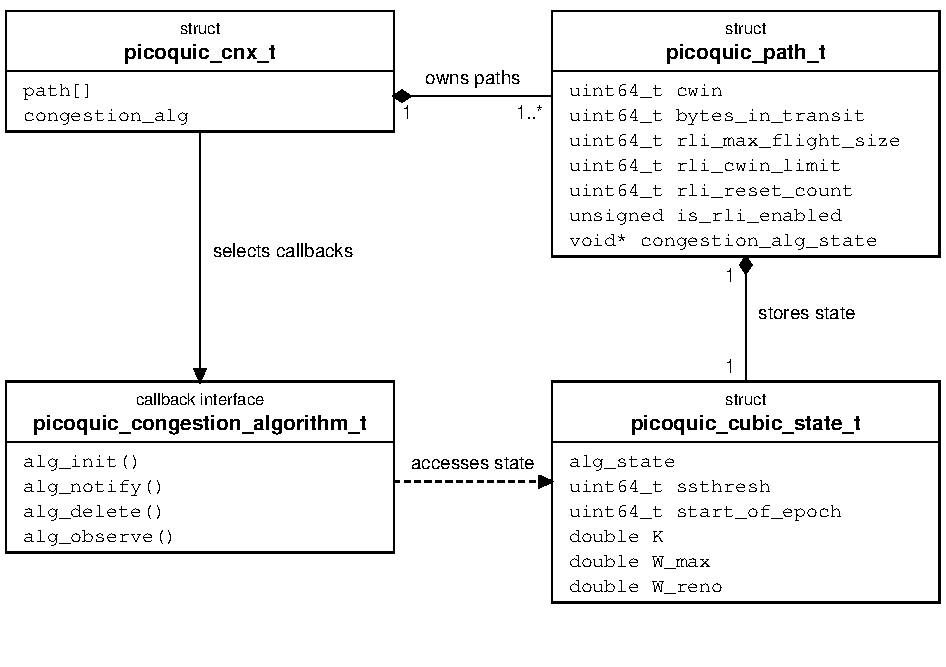
\includegraphics[width=\linewidth,height=0.48\textheight,keepaspectratio]{images/implementation-structure.pdf}
\captionof{figure}{Class-style structural diagram of the core C structs and callback interface. Selected fields are shown.}
\end{center}

picoquic\_cnx\_t holds path references and the selected congestion-control interface. A path holds cwnd, flight accounting, RLI fields, and an opaque pointer to its algorithm state. picoquic\_cubic\_state\_t remains the private CUBIC state. ACK information is passed through picoquic\_per\_ack\_state\_t to the notification callback. The diagram uses C struct and callback-interface stereotypes because the implementation is C; it does not invent C++ classes or member methods \cite{ref12}.


The sender module updates flight history where packet enqueue and dequeue accounting occurs. CUBIC computes limits, applies growth, and resets observation state during recovery. The logging modules export the resulting values. This distribution follows existing ownership: packet accounting remains in sender.c, policy remains in cubic.c, and diagnostics remain in the log writers and converters.


State is per path even though the live campaign selects one path. Focused tests create independent path instances to check isolation. That unit-level check does not establish correct live multipath behaviour, which would require dedicated connections and trace selection.


\subsection*{4.2 Initialization and packet accounting pseudocode}


\begingroup\footnotesize
\begin{verbatim}
ON_CUBIC_INITIALIZE(path, option):
    path.rli_enabled = option in {"rli", "rli=on", "on"}
    initialize_existing_CUBIC_state(path)
    path.cwnd = INITIAL_CWND
    path.maxFS = INITIAL_CWND if enabled else 0
    path.limit = 2 * INITIAL_CWND if enabled else 0
    path.reset_count = 0
    path.capped = false

ON_FLIGHTSIZE_UPDATE(path):
    if path.rli_enabled:
        path.maxFS = max(path.maxFS, path.bytes_in_transit)

ON_PACKET_ENQUEUE(path, packet_bytes):
    perform_existing_enqueue_and_flight_accounting()
    ON_FLIGHTSIZE_UPDATE(path)

ON_PACKET_DEQUEUE(path, packet):
    perform_existing_removal_and_flight_accounting()
    ON_FLIGHTSIZE_UPDATE(path)
\end{verbatim}
\endgroup

INITIAL\_CWND is 10 \(\times\) PICOQUIC\_MAX\_PACKET\_SIZE in this source, or 15,360 bytes in the recorded runs. Initializing maxFS to that value explains why a flight smaller than 15 KiB can still authorize growth toward 30 KiB in slow start. The maximum is not redefined as merely the largest small application frame. The source's send\_mtu is used for the additive congestion-avoidance limit.


\subsection*{4.3 Implementation map}

\begingroup\small\setlength{\tabcolsep}{4pt}\renewcommand{\arraystretch}{1.15}
\noindent\begin{tabular}{|>{\raggedright\arraybackslash}p{\dimexpr 0.33607\linewidth-2\tabcolsep-2\arrayrulewidth\relax}|>{\raggedright\arraybackslash}p{\dimexpr 0.66393\linewidth-2\tabcolsep-2\arrayrulewidth\relax}|}
\hline
\textbf{Source file / component} & \textbf{Implemented responsibility} \\ \hline
picoquic\_internal.h & Per-path RLI fields, flags, and reset counter. \\ \hline
sender.c & Maximum-flight accounting after enqueue and dequeue. \\ \hline
cubic.c & Activation, candidate growth, caps, epoch guard, recovery reset, and DCUBIC isolation. \\ \hline
logwriter.c; loglib/qlog*.c & Binary/direct qlog fields and optional-field conversion. \\ \hline
plot\_cwnd.py; experiments/*.py & Time-unit handling, trace parsing, graphs, validation, and campaign summaries. \\ \hline
\end{tabular}\endgroup
\par\vspace{0.6em}

Cap arithmetic saturates at UINT64\_MAX. Reset counting also saturates, avoiding wraparound in a long-running path. The Ubuntu verification did not separately exercise the overflow boundary.


\subsection*{4.4 Growth and reduction pseudocode}


\begingroup\footnotesize
\begin{verbatim}
ON_ACK_GROWTH(path, ack, phase):
    old = path.cwnd
    if not path.rli_enabled:
        run_existing_CUBIC_ACK_logic(); return
    candidate = existing_phase_candidate_with_RLI_growth(ack)
    limit = SAT_ADD(path.maxFS, path.send_mtu) if phase == CA
            else SAT_DOUBLE(path.maxFS)
    candidate = max(candidate, old)       # ACK cannot shrink cwnd
    path.capped = candidate > old and candidate > limit
    path.cwnd = max(old, min(candidate, limit))
    path.W_reno = min(path.W_reno, path.cwnd)
    path.limit = limit

ON_REAL_WINDOW_REDUCTION(path, congestion_event):
    run_existing_CUBIC_recovery_response(congestion_event)
    if path.rli_enabled:
        path.maxFS = 0; path.limit = 0; path.capped = false
        path.reset_count = SAT_ADD(path.reset_count, 1)
\end{verbatim}
\endgroup

The pseudocode summarizes the RLI logic and does not replace the existing ACK, recovery, or RTT state machine. The first live pilot exposed an ACK-driven decrease after an epoch adjustment. The corrected helper preserves the old window in that path. Genuine reductions still use recovery and clear maxFS. Spurious recovery may restore CUBIC window and epoch state, but does not restore the pre-reduction flight maximum \cite{ref12}.


\subsection*{4.5 Verification and instrumentation}

qlog exports rli\_max\_flight\_size, rli\_cwnd\_limit, rli\_capped, and rli\_reset\_count. The counter makes a reset observable when the flight has already rebuilt before the next snapshot. The trace validator rejects unreset decreases, uncapped growth, missing cap exercise, and maximum-flight values below observed flight. A retained peak above both adjacent samples is accepted as a possible intermediate event and counted, rather than incorrectly rejected.


\begingroup\small\setlength{\tabcolsep}{4pt}\renewcommand{\arraystretch}{1.15}
\noindent\begin{tabular}{|>{\raggedright\arraybackslash}p{\dimexpr 0.27049\linewidth-2\tabcolsep-2\arrayrulewidth\relax}|>{\raggedright\arraybackslash}p{\dimexpr 0.72951\linewidth-2\tabcolsep-2\arrayrulewidth\relax}|}
\hline
\textbf{Saved verification} & \textbf{Outcome and scope} \\ \hline
Full regression & Both registered CTest entries passed for both versions. The baseline ran 667 internal checks and the RLI build ran 668. \\ \hline
Focused C checks & The \texttt{cubic\_rli} test covered growth caps, packet accounting, loss, ECN, timeout, spurious recovery, and CUBIC epoch handling. \\ \hline
Live trace checks & All twelve RLI connections passed the applicable observed-invariant checks. \\ \hline
\end{tabular}\endgroup
\par\vspace{0.6em}

\label{sec:implementation-end}
